\message{ !name(implementation-and-results.tex)}
\message{ !name(implementation-and-results.tex) !offset(-2) }
\chapter{Implementation and Results}\label{cha:implementation}

\section{Front-end}\label{cha:implementation:sec:front-end}
\dots

\subsection{Component Structure}
\dots

\subsubsection{Services}
\dots
\subsubsection{Modules}
\dots
\subsubsection{Dialogs}
\dots
\subsection{Generic Form Control Builder}
\dots
\subsection{Spring HATEOAS Classes}
\dots
\subsubsection{Entity Class}
\dots
\subsubsection{Acessor Class}
\dots
\subsubsection{Repository Class}
\dots
\subsubsection{Repository Service Class}
\dots
\subsection{Temporal Caching Repository}
\dots
\subsection{Error Handler}
\dots
\subsection{Database Reader}
\dots

\section{Back-end}\label{cha:implementation:sec:back-end}
\dots

\subsection{Entities}
Following the class diagram in Figure~\ref{fig:classdiagram} and their relations, classes were created and properly annotated with so that \gls{JPA} is able to properly generate a relational model. Hence the \texttt{Entity} annotation is present in all classes.

Listing~\ref{code:sqlquery} presents the implementation of the Query model defined in Section~\ref{model:query}, it servers as an overview into other model implementations as it shares much of the common features but also adds some of its own.

Lines 1, 2 and 5 are provided by the Lombok package as discussed in Section~\ref{tech:lombok}, instructing the creation of constructor and other common methods during compilation. All models make use of \texttt{@Data} and \texttt{@NoArgsConstructor} annotations and all but \texttt{PermissionTree} uses \texttt{@AllArgsConstructor}.

In regards to \gls{ORM}, \texttt{@Entity} annotation in line 3 is the entry-point through which \gls{JPA} evaluates what classes are meant to be taken into account when building the relational model.
In general, some attributes need don't need to be declared as they are correctly inferred but in some cases it is desired to configure the generated database, \texttt{@Column} annotation on line 11 changes the default behavior so that the length of the corresponding \texttt{varchar} field in the table is able to hold larger amounts of characters; The other models, \texttt{YabiUser} \texttt{PermissionTree} and \texttt{Directory} make extensive use of \texttt{@Column} to specify columns that shouldn't have repeated values.

Relation between entities are made though \texttt{@OneToOne}, \texttt{@ManyToOne} and \texttt{@ManyToMany} annotations.
The first two represents single value association between entities, however, they represent different semantics and where the foreign key will be created.
\texttt{@ManyToOne} indicates that the foreign key will stay in the table in which this model is mapped to, \texttt{@OneToOne} makes no distinction, leaving for the \gls{ORM} back-end implementation to decide.
Line 17 is declaring that more that one instance of \texttt{SqlQuery} may reference a single \texttt{Directory} and that \texttt{SqlQuery} will hold the foreign key to \texttt{Directory}.
\texttt{@ManyToMany} represents a collection of associations, here used to associate \texttt{YabiUser} to \texttt{PermissionTree} so that many users can have many, overlapping, permissions. One possible parameter to \texttt{@ManyToMany} is the \texttt{FetchType}, instructing the \gls{ORM} engine to retrieve the associated entity only when it is accessed or together with its parent is retrieved.

\texttt{@JoinColumn} annotation is a general purpose configuration for relational fields, in line 18 and 22 it's used to configure the name in which the column will be called and whether it can have no specified value.

\lstinputlisting[firstline=22,float,
caption=Implementation of the Query model,
label=code:sqlquery
]{listings/SqlQuery/SqlQuery.java}

The remaining entities follow a similar pattern in it's implementation.

\subsection{Spring Configuration}
This section presents Spring configurations that took place so that \gls{Yabi} is able to work as expected. In order for Spring Framework to stay out of the way as much as it can and allow developers to focus on the implementation of business functionalities, it makes many assumptions about how its components interact, however, at some point the application being developed grow some needs that conflict with Spring defaults. When this eventually happens, which was the case with \gls{Yabi}, developers can override some of Spring's default behavior by implementing specific interfaces.



\subsubsection{Security}
\gls{Yabi}'s security model uses a directory server to authenticate and a relational database to load user roles and execute authorization checks. Because this is a stateless application, every request follows the steps shown in Figure~\ref{fig:authseq} before being executed by the controllers.

Authentication is done through a anonymous bind to a \gls{LDAP} server, Section~\ref{impl:ldap} goes through the Spring configuration necessary to make it work and Section~\ref{impl:detailsmapper} explains how the roles are loaded into the Sprig Security's \texttt{UserDetails} object.

In regards to authorization, there are two possible roles in which a use must be assigned to, either \texttt{ADMIN} or \texttt{USER}. With this, non-administrative resources are simply not dependent on the user's role therefore accessible to all users, meanwhile, administrative resources are explicitly marked to be accessible by users whose role is \texttt{ADMIN}, more on this in Section~\ref{impl:admres}.

Figure~\ref{fig:authseq}, presents in a general view the steps taken to authenticate and load an user's details. It is infeasible to model the whole of Spring Web and Spring Security as it is quite a extensive feature and it is out of the scope of this report, therefore it was abstracted into fewer elements, namely \texttt{WebSecurity} entity representing the objects that gets built by the configuration shown in Listing~\ref{code:authblock}, the \textit{authenticate} message is abstracting Spring's authentication provider voting system, \texttt{LDAP AuthenticationManager} entity representing \gls{LDAP}'s \texttt{AuthenticationProvider} and \textit{anonymous bind}, as the name implies is the authentication that takes place in the directory server.

The main point of Figure~\ref{fig:authseq} is to show that once the bind takes place in the \texttt{LDAP AuthenticationManager}, the library requests an object that implements the \texttt{UserDetailsContextMapper} to populate it's newly created \texttt{Authentication} object with business-specific information in the form of a \texttt{UserDetails}. In this case \texttt{YabiUserDetailsManager} is chosen by Spring's dependency injection mechanism and it provides an instance of \texttt{YabiUser}, which implements \texttt{UserDetails} interface, that is retrieved from \gls{Yabi}'s database.

\begin{figure}
  \centering
  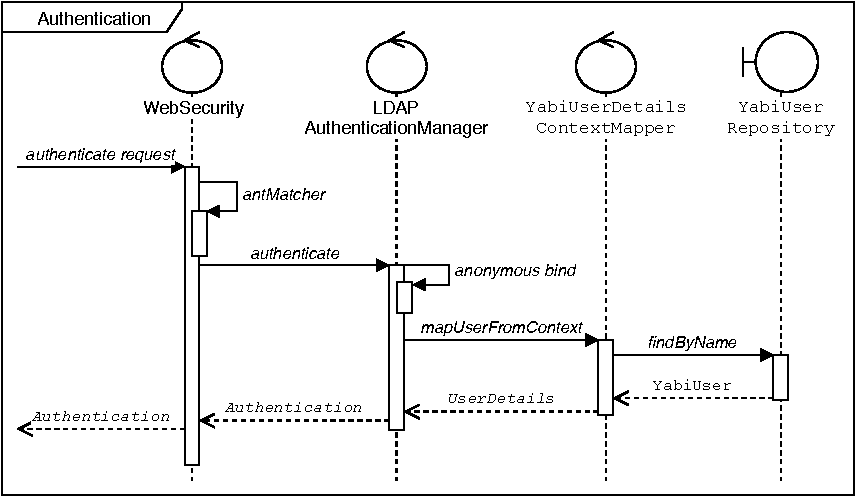
\includegraphics[width=.9\textwidth]{images/diagramas/authentication}
  \caption{Authentication Sequence Diagram}\label{fig:authseq}
\end{figure}


\subsubsection{Admin Resources}\label{impl:admres}
Not all endpoints are freely accessed to all users because they involve possibly destructive interactions with the information contained in the system. In this implementation, non-administrative users get their information through custom \texttt{RestController} that expose fewer functionalities and administrative users may directly request the repositories. Repositories are further discussed in Section~\ref{impl:repos}.

Suffice to say that certain endpoints require the user to be authenticated and to have an administrator role. Listing~\ref{code:authblock} is the configuration that enforces this statement.

The call to \texttt{antMatchers} in lines 47, 49 and 51 works by specifying a list of \gls{HTTP} paths and applying some definitions or restrictions whenever an incoming request is a member of it. \todo{membro da lista de caminhos http}. In this specific case, all requests to repositories are eligible to continue only if the \texttt{hasRole} definition evaluates to true.

Line 51 is protecting the \textbf{/permission} endpoint from being requested with a \gls{HTTP} \textsc{delete} verb.
Lines 46 and 52 declare that all \gls{HTTP} requests are to be authenticated.

\todo{as linhas estao certas ?}
\lstinputlisting[firstline=39, lastline=55, float,
caption=HttpSecurity configuration,
label=code:authblock
]{listings/Configuration/SecurityConfiguration.java}

\subsubsection{\gls{CORS} Mapping}

Because \gls{Yabi} is a web \gls{API} and a front-end application, it is necessary that both parties can interact but due to security reasons, most browsers implementations block \gls{AJAX} calls if the remote server does not explicitly add the current domain to it's response header.

In Spring, specifying allowing domains to access it's resources is done by implementing the \texttt{WebMvcConfigurer}, overriding the method \textit{addCorsMapping(CorsRegistry)} and calling \textit{allowedOrigins} on it's parameter. The method \textit{allowedOrigins} takes a list of stings that contain valid \gls{URL} addresses.

\gls{Yabi} configures this using the \texttt{application.properties} file under the key \texttt{yabi.web.allowedOrigins}, allowing for a centralized configuration.

\subsubsection{\gls{LDAP}}\label{impl:ldap}

Following the authentication specification in Section~\ref{proj:auth}, Listing~\ref{code:ldapauth} presents the configuration that implements the desired behavior.

\lstinputlisting[firstline=57, lastline=66, float,
caption=LDAP Authentication Configuration,
label=code:ldapauth
]{listings/Configuration/SecurityConfiguration.java}

\todo{checar linhas no listing gerado}
In this configuration, \texttt{AuthenticationManagerBuilder} is a class used by Spring in it's security pipeline. It comes with built-in support for \gls{LDAP}, \gls{JDBC} and in-memory authentication mechanisms; line \todo{4} is declaring \gls{LDAP} authentication to be used.

Line \todo{5} is considered important because it is mapping a custom details context mapper to the authentication pipeline. What this does is to provide a hook in the authentication pipeline to allow explicit customization of the user object after it is authenticated. The given mapper, \texttt{YabiUserDetailsContextMapper} retrieves the authenticated user's instance of \texttt{YabiUser}.

Lines \todo{6 to 9} configure the connection to the remote directory service, including it's address and what to bind with.

\subsubsection{User Details Context Mapper}\label{impl:detailsmapper}
Often times a directory service is used as an authentication mechanism. Applications issue an anonymous bind request to the server passing their user's credentials and if properly found and matched, a boolean value is returned, however, applications often has information about the user that must be sent accessible to other parts of the framework. To do so, Spring Security utilizes this interface to retrieve a \texttt{UserDetails} instance that gets injected into the commonly accessible \texttt{Authentication} interface.

For this application, a new implementation of the \texttt{UserDetailsContextMapper} interface is provided, \texttt{YabiUserDetailsContextMapper} returns an instance of \texttt{YabiUser}, which implements said \texttt{UserDetails} interface and adds \gls{Yabi}-specific attributes, enabling other parts of the system to query the current user's related information such as their role, \texttt{PermissionTree} and name. More information about the \texttt{YabiUser} class is found in Section~\ref{model:user}.

\subsection{Custom Controllers \& View Models}
\texttt{RestController} is a Spring Web annotation that enables a given class or method to handle \gls{HTTP} requests. In essence it is a combination of two other annotations, the \texttt{Controller}, which is what trigger the framework into considering the class as a possible resolver of  \gls{HTTP} requests and \texttt{ReponseBody}, that wraps the method call into a response body. In simple cases the returned Object is mapped to a \gls{JSON} string.

Because the \texttt{PermissionTree} class contains a reference to it's parent, and the root references itself, there was a need to circumvent a infinite loop during it's \gls{JSON} serialization. To do so, rather simple and 
serializable classes whose role were to convey information to the front-end were written, namely, \texttt{SqlQueryViewModel}, \texttt{PermissionTreeViewModel} and \texttt{YabiUserViewModel}.

To accommodate the special handling of \texttt{PermissionTree} model and provide some custom functionalities some custom \texttt{RestController} were implemented, \texttt{SqlQueryController}, \texttt{PermissionTreeController} \texttt{YabiUserController} and \texttt{DatabaseReaderController}.

Filtering in relation to \texttt{Permission} was required when providing \texttt{SqlQuery} and \texttt{PermissionTree} objects to non-administrative users, it was implemented by iterating over the current user's permissions and appending all the elements under that permission to a list. Listing~\ref{code:queries} presents the implementation of such filtering applied to \texttt{SqlQuery} model.

\lstinputlisting[firstline=27,lastline=39, float,
caption=\textbf{/queries} Endpoint,
label=code:queries
]{listings/SqlQuery/SqlQueryController.java}

\subsubsection{DatabaseReaderController}
The retrieval of information contained in a remote database is exposed through the \texttt{DatabaseReaderController}. It's a wrapper to \texttt{DatabaseReader.runQuery} method that does a permission check before executing.

\subsubsection{PermissionTreeController}
Because of it's tree-like nature, once a \texttt{PremissionTree} is deleted, all of it's child nodes need also to be removed. However, because it reference its parent but not its children, leaving the \gls{RDBMS} to execute a cascading delete would eventually delete the root node. Therefore the \texttt{PermissionTreeController} implements the desired behavior on deletion. It is bound to a \gls{HTTP} \textsc{delete} verb on the path \textbf{/pemrission/\{id\}} 

\subsubsection{YabiUserController}
To provide the front-end with information about the current user, \texttt{YabiUserController} replies to \textsc{get} requests on the path \textbf{/user} with information contained inside the \texttt{Authentication} and thus avoid reaching out to the database a second time.

\subsection{Spring Repositories}\label{impl:repos}
\texttt{PagingAndSortingRepository} were created for all entities evaluated during the project phase, discussed thoroughly in Section~\ref{tities}. In this section an overview of the customizations done for each repository will be shown.

\subsubsection{YabiUserRepository}
After binding in the directory service, the application uses \texttt{YabiUser}

\subsection{ORM Generated Database}
\dots
\subsection{Multi-Database Support}
\dots

\section{Development Environment}\label{cha:implementation:sec:development}
\dots

\subsection{Apache Directory}
\dots
\subsection{Multi-Database Support}
\dots
\subsubsection{Microsoft SQL Server Docker Image}
\dots
\subsubsection{Oracle:XE Driver Access}
\dots
\subsection{Testing File}
\dots
\subsection{Postman Tests}
\dots


\message{ !name(implementation-and-results.tex) !offset(-184) }
